\documentclass[handout,compress]{beamer}

\usetheme[block=fill]{metropolis}

\usepackage{graphicx} % Allows including images
\usepackage{amsmath,amsfonts,amsthm,amssymb}
\usepackage{color}
\usepackage{xcolor,cancel}
%\setitemize{label=\usebeamerfont*{itemize item}%
%	\usebeamercolor[fg]{itemize item}
%	\usebeamertemplate{itemize item}}
\definecolor{mDarkBrown}{HTML}{604c38}
\definecolor{mDarkTeal}{HTML}{23373b}
\definecolor{mLightBrown}{HTML}{EB811B}
\definecolor{mMediumBrown}{HTML}{C87A2F}
\definecolor{mygreen}{HTML}{98C2B9}
\definecolor{myyellow}{HTML}{DFD79C}
\definecolor{myblue}{HTML}{8CA7CC}
\definecolor{kern}{HTML}{8CC2B7}

\usepackage{float}
\usepackage{framed}
\usepackage{epsfig}
\usepackage{graphicx}
\usepackage{subcaption}
\usepackage{ulem}
\usepackage{hhline}
\usepackage{multirow}
\usepackage{comment}   
\usepackage{bbm}
\usepackage{tikz}   
\usepackage{ulem}
\def\Put(#1,#2)#3{\leavevmode\makebox(0,0){\put(#1,#2){#3}}}
\newcommand*\mystrut[1]{\vrule width0pt height0pt depth#1\relax}
\newcommand{\eqdef}{\mathbin{\stackrel{\rm def}{=}}}


\newcommand{\bs}[1]{\boldsymbol{#1}}
\newcommand{\bv}[1]{\mathbf{#1}}
\newcommand{\R}{\mathbb{R}}
\newcommand{\E}{\mathbb{E}}

\DeclareMathOperator*{\argmin}{arg\,min}
\DeclareMathOperator*{\argmax}{arg\,max}
\DeclareMathOperator{\nnz}{nnz}
\DeclareMathOperator{\Var}{Var}
\DeclareMathOperator{\sinc}{sinc}
\DeclareMathOperator{\mv}{mv}
\DeclareMathOperator{\sgn}{sgn}
\DeclareMathOperator{\step}{step}
\DeclareMathOperator{\gap}{gap}
\DeclareMathOperator{\poly}{poly}
\DeclareMathOperator{\tr}{tr}
\DeclareMathOperator{\orth}{orth}
\newcommand{\norm}[1]{\|#1\|}
\captionsetup[subfigure]{labelformat=empty}
\captionsetup[figure]{labelformat=empty}
\DeclareMathOperator*{\lmin}{\lambda_{min}}
\DeclareMathOperator*{\lmax}{\lambda_{max}}

\newcommand{\specialcell}[2][c]{%
  \begin{tabular}[#1]{@{}c@{}}#2\end{tabular}}
\newcommand{\specialcellleft}[2][c]{%
\begin{tabular}[#1]{@{}l@{}}#2\end{tabular}
}

\usepackage{tabstackengine}
\stackMath

\newtheorem{claim}[theorem]{Claim}


%----------------------------------------------------------------------------------------
%	TITLE PAGE
%----------------------------------------------------------------------------------------

\title{CS-UY 4563: Lecture 14 \\ Support Vector Machines}
\author{NYU Tandon School of Engineering, Prof. Christopher Musco}
\date{}

\begin{document}

\begin{frame}
	\titlepage 
\end{frame}

\metroset{titleformat=smallcaps}

\begin{frame}
	\frametitle{course logistics}
	\begin{itemize}
		\item Project topic/teams due on \textbf{Wednesday} via email.
		\begin{itemize}
			\item Sign up for a meeting time after you send me the email.
		\end{itemize}
		\item Lab \texttt{lab\_grad\_descent\_partial.ipynb} due \textbf{Thursday night}.
		\begin{itemize}
			\item  We don't have enough time to do the topic of optimization justice, so take my class next semester if you want to learn more. 
		\end{itemize}
	\end{itemize}
	
\end{frame}

\begin{frame}
	\frametitle{last lecture}
	\begin{center}
	How to use \textbf{\alert{non-linear kernels}} with logistic regression. 
\end{center}
\begin{itemize}
	\item Often leads to better classification than basic linear logistic regression.
	\item Equivalent to feature transformation, but often computationally faster.
\end{itemize}
\end{frame}

\begin{frame} 
	\frametitle{examples of non-linear kernels}
	Commonly used positive semidefinite (PSD) kernel functions:
	\begin{itemize}
		\item Linear (inner-product) kernel: $k(\vec{x}, \vec{y}) = \langle \vec{x},\vec{y}\rangle$
		\item Gaussian RBF Kernel: $k(\vec{x}, \vec{y}) = e^{-\|\vec{x} - \vec{y}\|_2^2/\sigma^2}$
		\item Laplace Kernel: $k(\vec{x}, \vec{y}) = e^{-\|\vec{x} - \vec{y}\|_2/\sigma}$
		\item Polynomial Kernel: $k(\vec{x}, \vec{y}) = (\langle \vec{x},\vec{y}\rangle + 1)^q$.
	\end{itemize}
	\textbf{Recall:} Every PSD kernel has a corresponding feature transformation $\phi: \R^d \rightarrow \R^m$.
	\begin{align*}
		k(\vec{x}, \vec{y}) = \phi(\vec{x})^T\phi(\vec{y})) 
	\end{align*}
\end{frame}

\begin{frame} 
	\frametitle{kernel functions and feature transformation}
	\small
	\begin{center}
		Sometimes $\phi(\vec{x})$ is simple and explicit. \textbf{More often, it is not.}
	\begin{align*}
	\vec{x} &= \begin{bmatrix}x_1\\x_2\\x_3\end{bmatrix} & \phi(\vec{x}) &= \begin{bmatrix}1\\ \sqrt{2}x_1\\\sqrt{2}x_2\\\sqrt{2}x_3 \\ x_1^2 \\ x_2^2 \\ x_3^2 \\ \sqrt{2}x_1x_2 \\ \sqrt{2}x_1x_3 \\ \sqrt{2}x_2x_3\end{bmatrix}  
	\end{align*}
	Degree 2 polynomial kernel, $k(\vec{x},\vec{w}) = (\vec{x}^T\vec{w} + 1)^2$.
	\end{center}
\end{frame}

\begin{frame} 
	\frametitle{kernel matrix}
	Typically doesn't matter because we \emph{only need} to compute the \emph{kernel Gram matrix} $\bv{K}$ to retrofit algorithms like logistic or linear regression to use non-linear kernels. 
	\begin{center}
		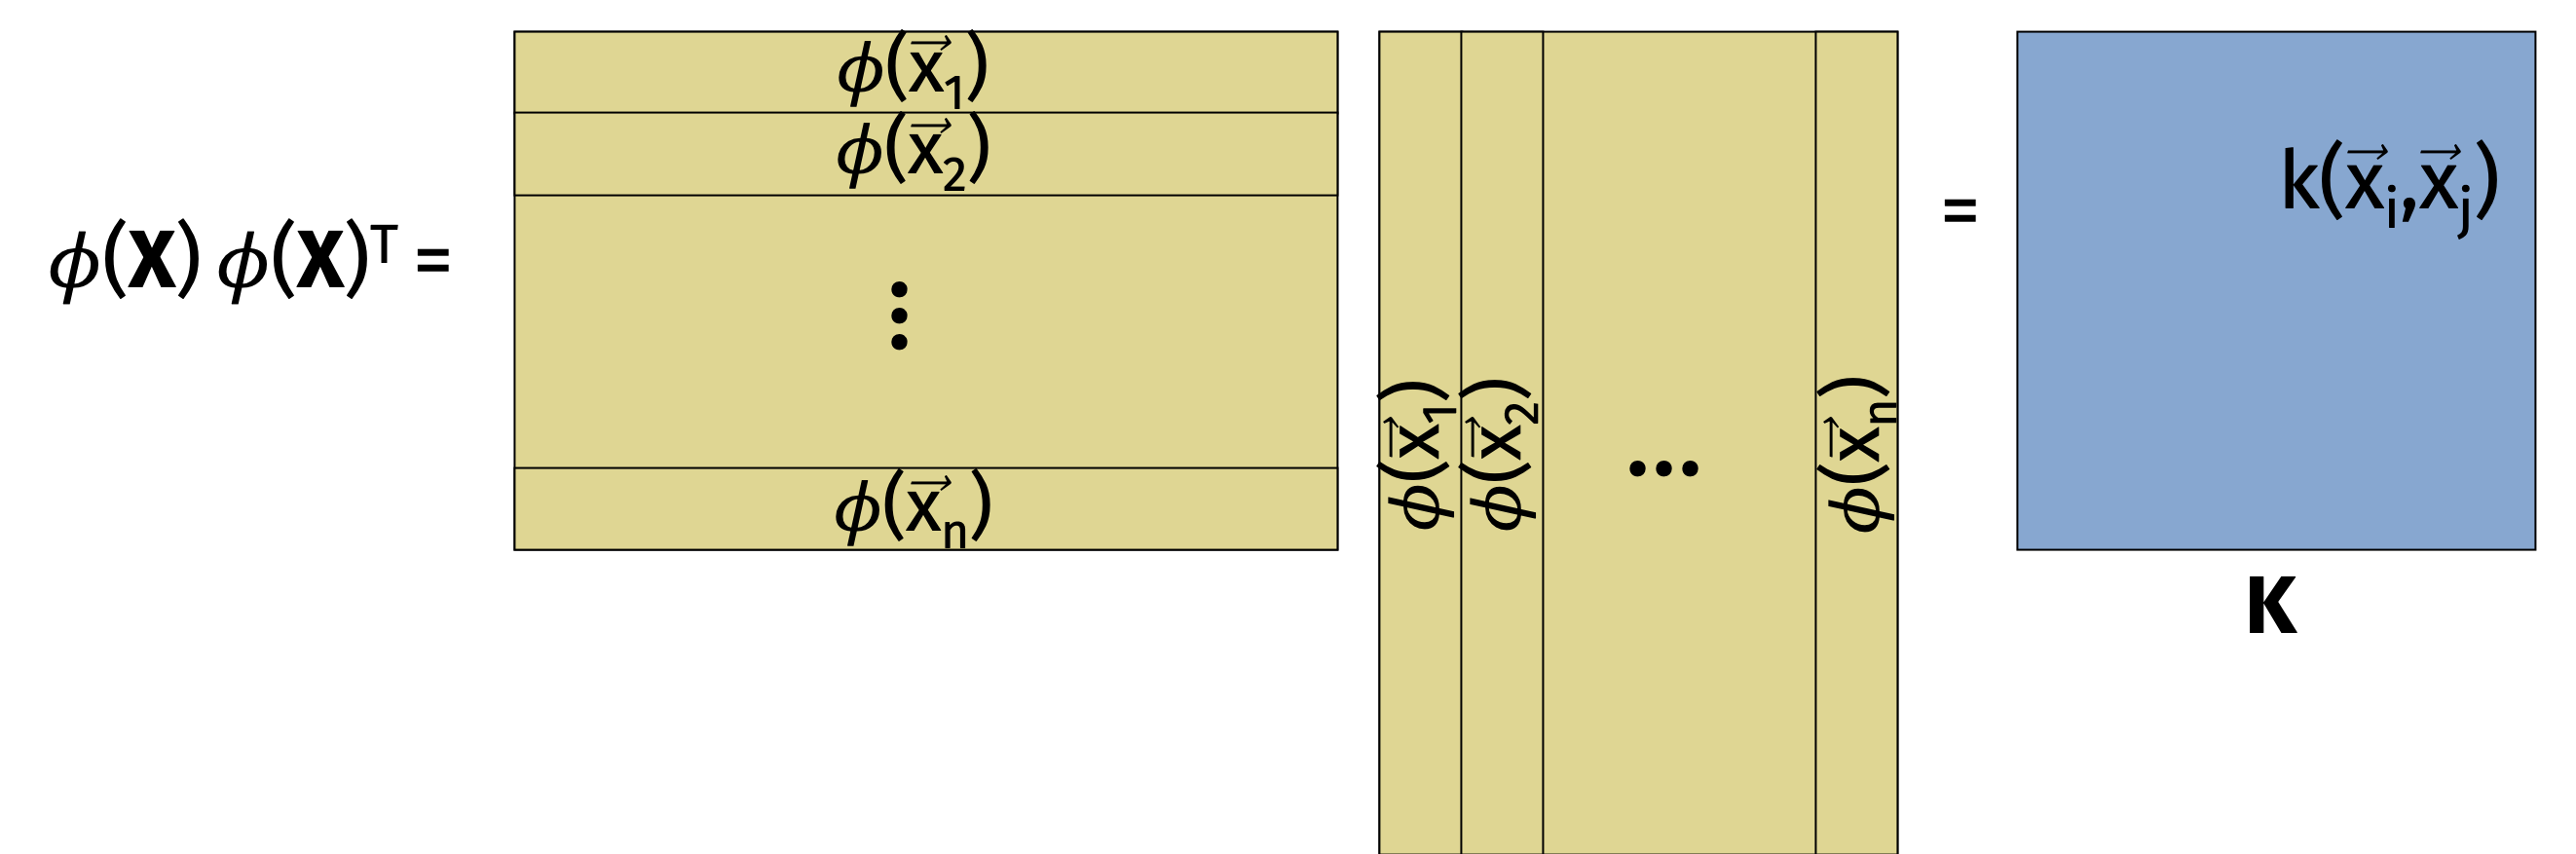
\includegraphics[width=\textwidth]{kernel_matrix.png}
	\end{center}
	\footnotesize{(If this stuff interests you, understanding the kernel feature maps $\phi$ which correspond to different kernels is a large part of my current research. This understanding can lead to faster kernel methods.)}
\end{frame}

\begin{frame} 
	\frametitle{today}
	\textbf{Support Vector Machines (SVMs)}:
	Another algorithm for finding \emph{linear classifiers} which is as popular as logistic regression. 
	\begin{itemize}
		\item Can also be combined with kernels.
		\item Developed from a pretty different perspective.
		\item But final algorithm is not that different. 
	\end{itemize}

\begin{columns}
	\begin{column}{.5\textwidth}
		\centering
		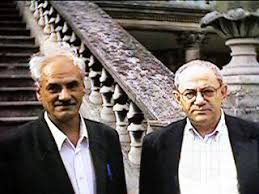
\includegraphics[width=.8\textwidth]{vc.jpeg}
	\end{column}
	\begin{column}{.5\textwidth}
		\small
		\begin{itemize}
		\item Invented in 1963 by Alexey Chervonenkis and Vladimir Vapnik. Also founders of VC-theory.
		\item First combined with non-linear kernels in 1993. 
		\end{itemize}
	\end{column}		
\end{columns}
\end{frame}

\begin{frame}
	\frametitle{svm's vs. logistic regression}
	For some reason, SVMs are more commonly used with non-linear kernels. For example, \texttt{sklearn}'s SVM classifier (called SVC) has support for non-linear kernels built in by default. Its logistic regression classifier does not. 
	
	\begin{itemize}
		\item I believe this is \emph{mostly} for historical reasons and connections to theoretical machine learning.
		\item In the early 2000s SVMs where a ``hot topic'' in machine learning and their popularity persists.
		\item It is not clear to me if they are better than logistic regression, but honestly I'm not sure... 
	\end{itemize}
\end{frame}

\begin{frame}
	\frametitle{svm's vs. logistic regression}
	\centering
	Next lab: \texttt{lab\_mnist\_partial.ipynb}. 
	\begin{center}
		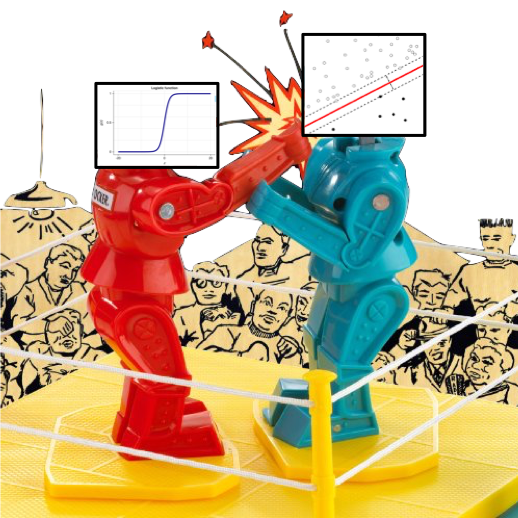
\includegraphics[width=.4\textwidth]{faceoff.png}
	\end{center}
	Machina-a-machina comparison of SVMs vs. logistic regression for a MNIST digit classification problem. Which provides better accuracy? Which is faster to train? 
	
	\textbf{20\% extra credit} on lab if you can beat my simple baseline.
\end{frame}

\begin{frame}
	\frametitle{linearly separable data}
	We call a dataset with binary labels \emph{linearly separable} if it can be perfectly classified with a linear classifier:
	\begin{center}
		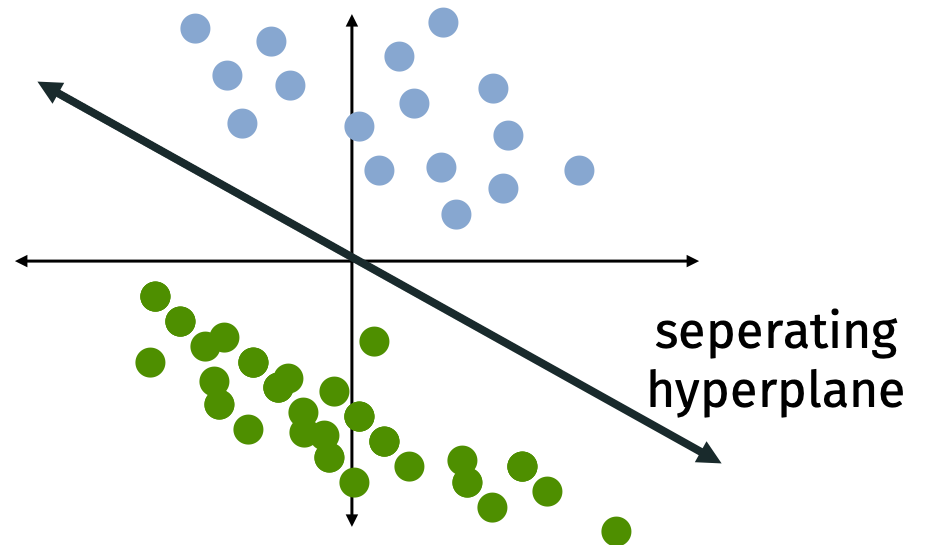
\includegraphics[width=.6\textwidth]{linearly_seperable.png}
	\end{center}
\end{frame}

\begin{frame}
	\frametitle{linearly separable data}
	Formally, there exists a parameter $\vec{\beta}$ such that $\langle\vec{\beta}, \vec{x}\rangle > 0$ for all $\vec{x}$ in class $1$ and $\langle\vec{\beta}, \vec{x}\rangle < 0$ for all $\vec{x}$ in class $0$.
	\begin{center}
		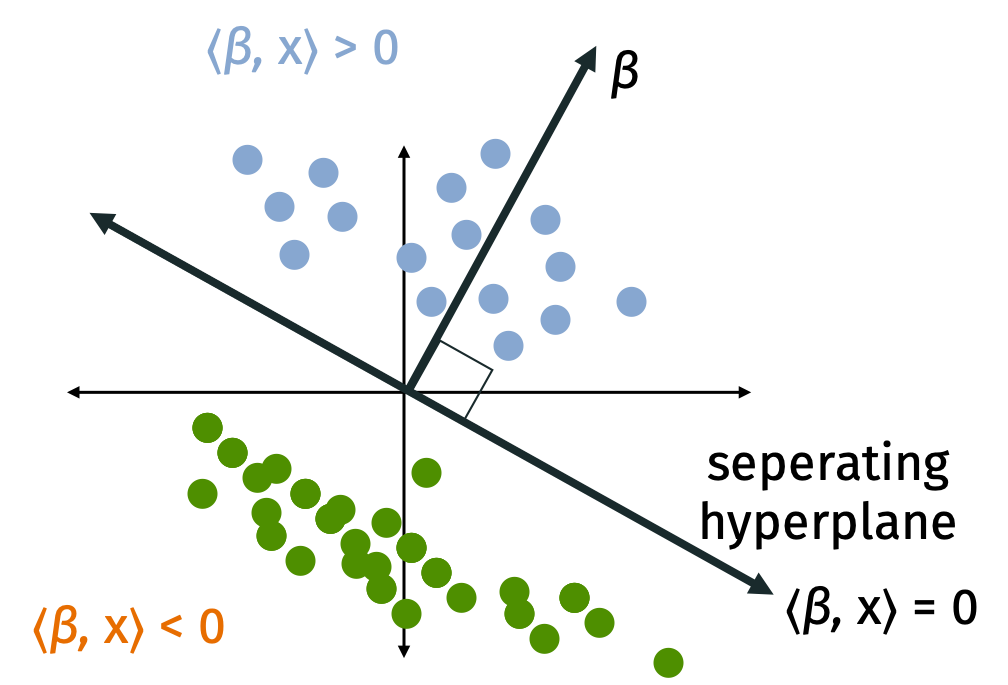
\includegraphics[width=.6\textwidth]{linear_seperable_math.png}
	\end{center}
	Note that if we multiply $\vec{\beta}$ by any constant $c$, $c\vec{\beta}$ gives the same separating hyperplane because $\langle c\vec{\beta}, \vec{x}\rangle = c\langle\vec{\beta}, \vec{x}\rangle$. 
\end{frame}

\begin{frame}
	\frametitle{linearly separable data}
	A data set might be linearly separable when using a non-kernel/feature transformation even if it is not separable in the original space.
	\begin{center}
		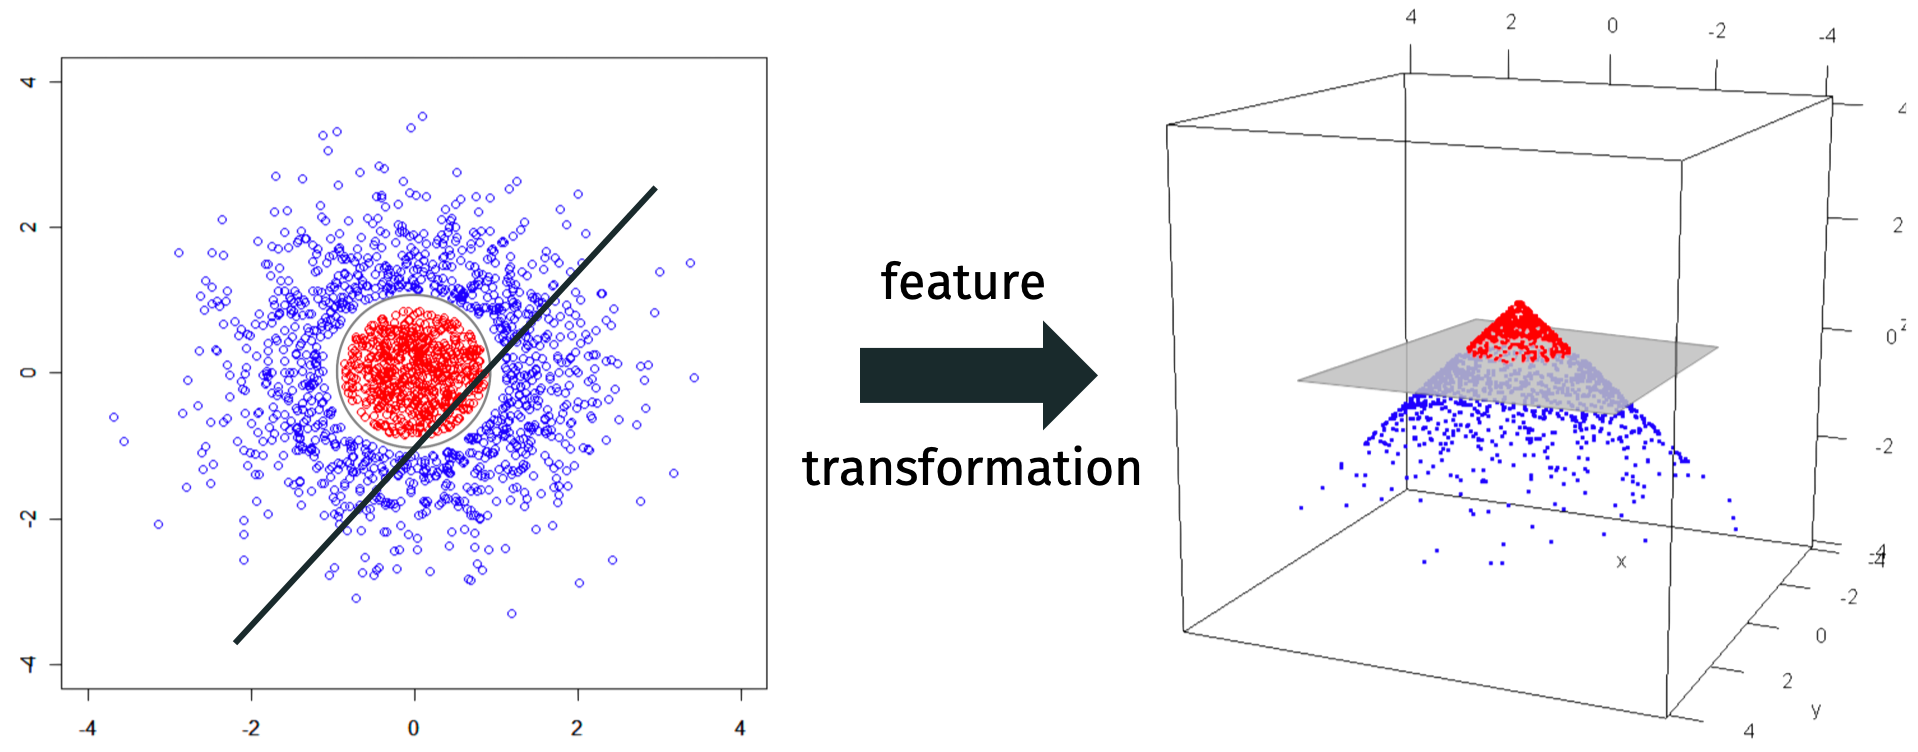
\includegraphics[width=.8\textwidth]{kernel_vis.png}
		
		This data is separable when using a degree-$2$ polynomial kernel. If suffices for $\phi(\vec{x})$ to contain $x_1^2$ and $x_2^2$. 
	\end{center}
\end{frame}

\begin{frame}
	\frametitle{margin}
	\centering
	When data is linearly separable, there are typically multiple valid separating hyperplanes.
	
	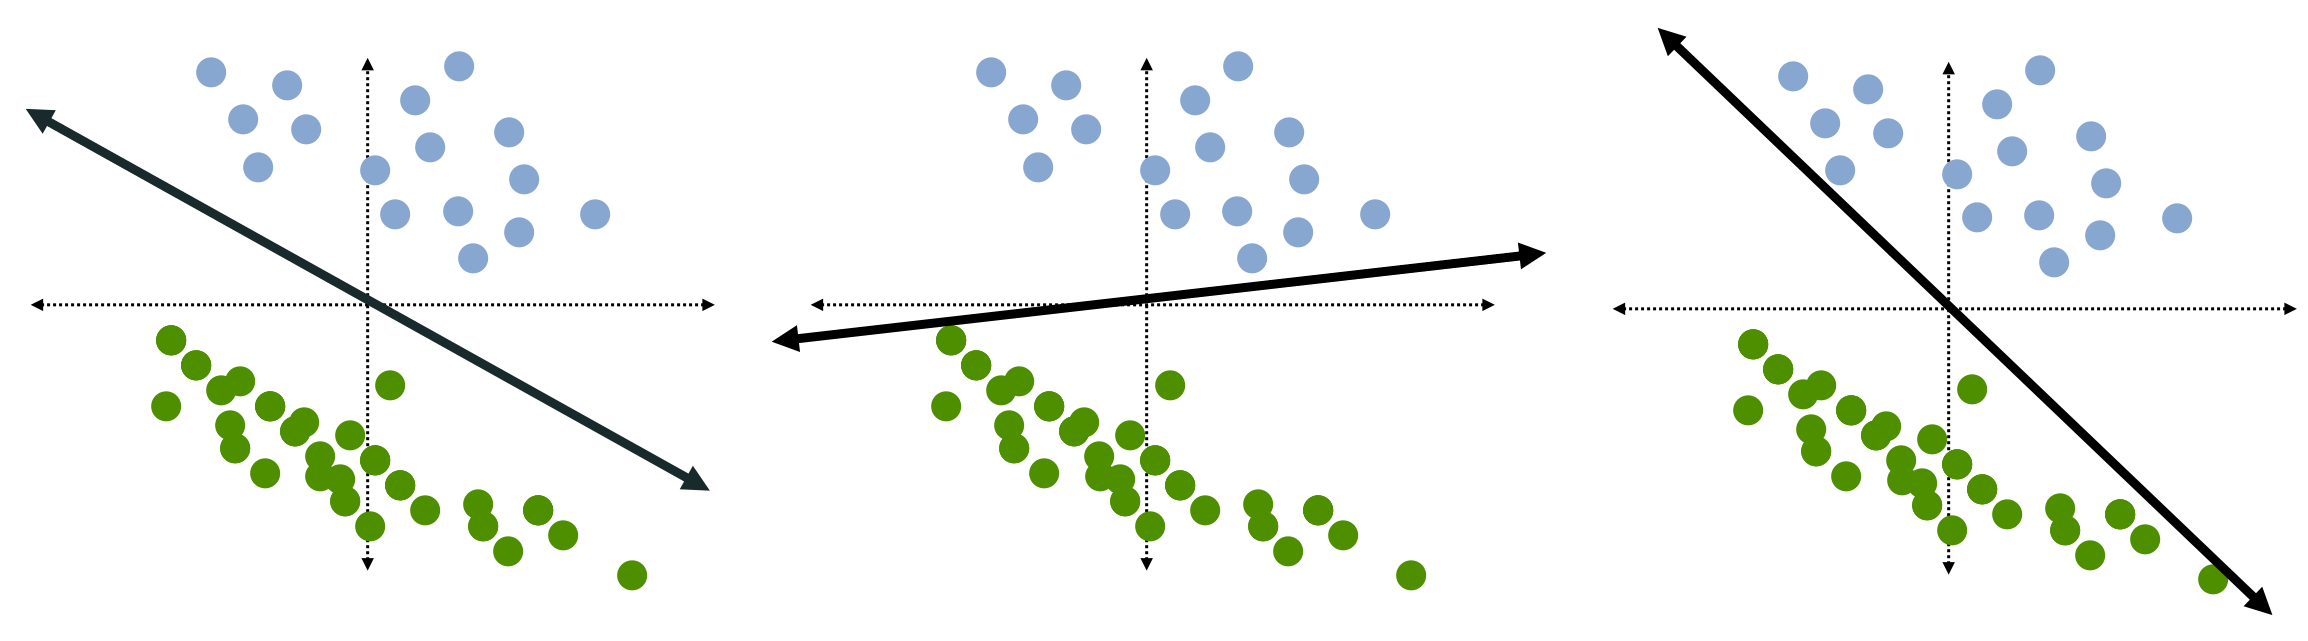
\includegraphics[width=\textwidth]{multiple_lines.png}
	
	\textbf{{Which hyperplane/classification rule is best?}}
\end{frame}

\begin{frame}
	\frametitle{margin}
	The \textbf{margin} $m$ of a separating hyperplane is the \emph{minimum} $\ell_2$ (Euclidean) distance between a point in the dataset and the hyperplane.
	\begin{center}
		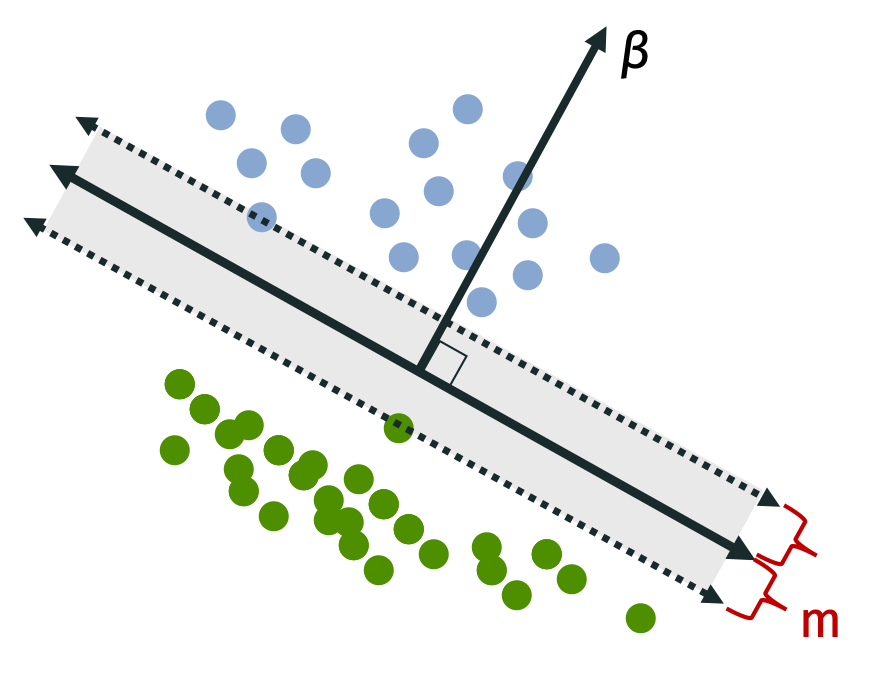
\includegraphics[width=.5\textwidth]{margin.png}
	\end{center}
	\begin{align*}
		m &= \min_i \Delta_i & &\text{where} & \Delta_i &= \frac{|\langle\vec{x}_i, \vec{\beta}\rangle|}{\|\vec{\beta}\|_2}
	\end{align*}
\end{frame}

\begin{frame}
	\frametitle{support vector}
	A \textbf{support vector} is any data point $\vec{x}_i$ such that $\frac{|\langle\vec{x}_i, \vec{\beta}\rangle|}{\|\vec{\beta}\|_2} = m$. 
	\begin{center}
		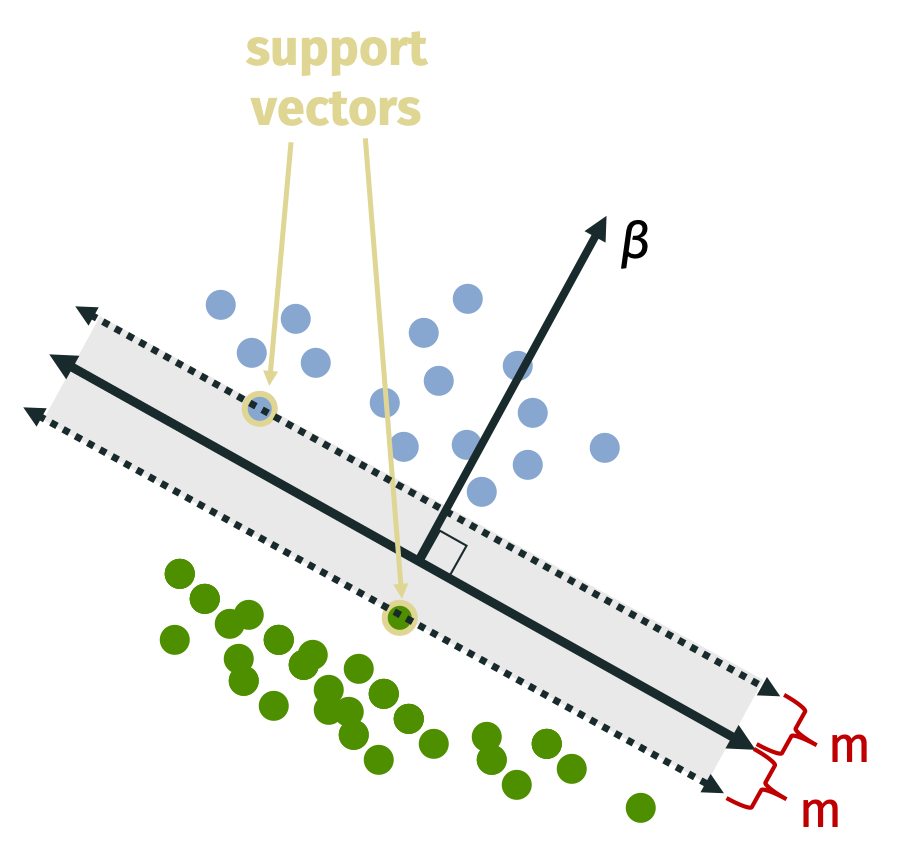
\includegraphics[width=.5\textwidth]{support_vector_hard.png}
	\end{center}
\end{frame}

\begin{frame}
	\frametitle{hard-margin svm}
	A \emph{hard-margin} support vector machine (SVM) classifier finds the \textbf{maximum margin (MM) linear classifier}.
	\begin{center}
		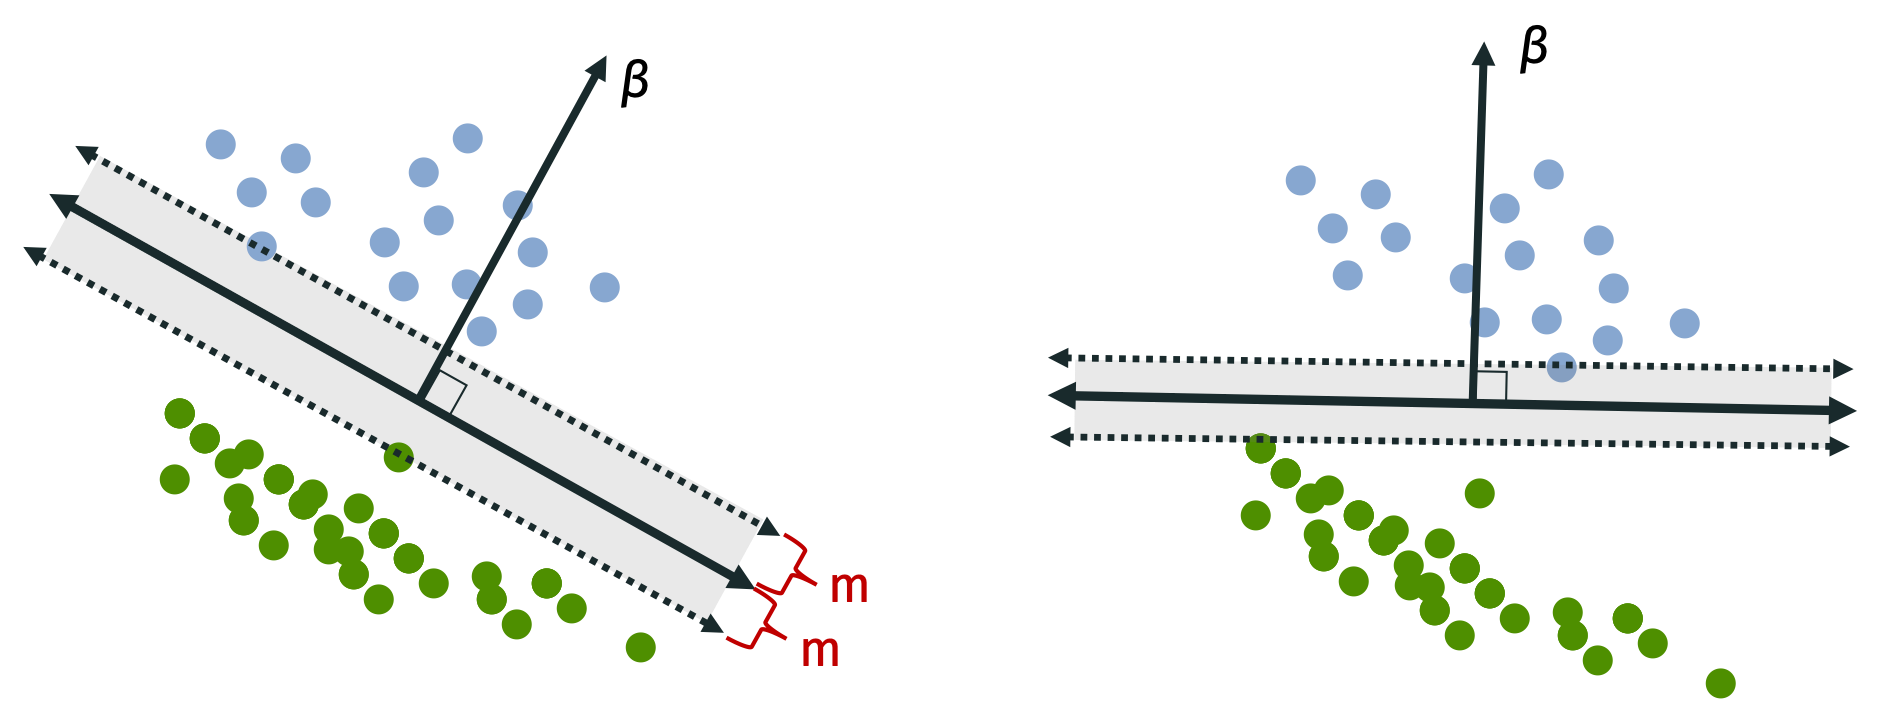
\includegraphics[width=.8\textwidth]{max_margin.png}
	\end{center}
 I.e. the separating hyperplane which {maximizes the margin $m$}.
\end{frame}

\begin{frame}
	\frametitle{margin}
	Denote the maximum margin by $m^*$. 
	\begin{align*}
	m^* &= \max_{\vec{\beta}} \left[\min_{i\in 1, \ldots, n} \frac{|\langle |\vec{x}_i, \beta\rangle|}{\|\vec{\beta}\|_2} \right]\\
	&= \max_{\vec{\beta}} \left[\min_{i\in 1, \ldots, n} \frac{y_i\cdot\langle \vec{x}_i, \vec{\beta}\rangle}{\|\vec{\beta}\|_2} \right]
%	&=  \max_{\vec{\beta}, \|\vec{\beta}\|_2 \leq 1} \left[\min_{i\in 1, \ldots, n} |\langle |\vec{x}_i, \beta\rangle|\right] \\
%	&=  \max_{\vec{\beta}, \|\vec{\beta}\|_2 \leq 1} \left[\min_{i\in 1, \ldots, n}  y_i\cdot\langle \vec{x}_i, \vec{\beta}\rangle\right]
	\end{align*}
	where $y_i = -1,1$ depending on what class $\vec{x}_i$.\footnote{Note that this is a different convention than the $0,1$ class labels we typically use.}
\end{frame}

%\begin{frame}
%	\frametitle{hard-margin svm}
%	A \emph{hard-margin} support vector machine classifier finds the separating hyperplane which \emph{maximizes the margin $m$}:
%	\begin{align*}
%		&\max_{\vec{\beta}} \underbrace{\left[\min_{i\in 1, \ldots, n} y_i\cdot\langle \vec{x}_i, \vec{\beta}\rangle\right]}_{\text{scaled margin}}] & &\text{subject to}  & \|\vec{\beta}\|_2 &\leq 1.
%	\end{align*}
%\end{frame}

\begin{frame}
	\frametitle{hard-margin svm}
	Equivalent formulation:
	\begin{align*}
	&\min_{\vec{\beta}} \|\vec{\beta}\|_2^2 & &\text{subject to}  & y_i\cdot\langle \vec{x}_i, \vec{\beta}\rangle &\geq 1 \text{ for all } i.
	\end{align*}
	Under this formulation $m = \frac{1}{\|\beta\|_2}$.
	\vspace{9em}
	
	
	This is a \textbf{constrained optimization problem.} In particular, a \emph{linearly constrained quadratic program}, which is a type of problem we have efficient optimization algorithms for. 
\end{frame}

\begin{frame}
	\frametitle{hard-margin svm}
	\small
	While important in theory, hard-margin SVMs have a few critical issues in practice:
	\begin{center}
		\vspace{-1em}
		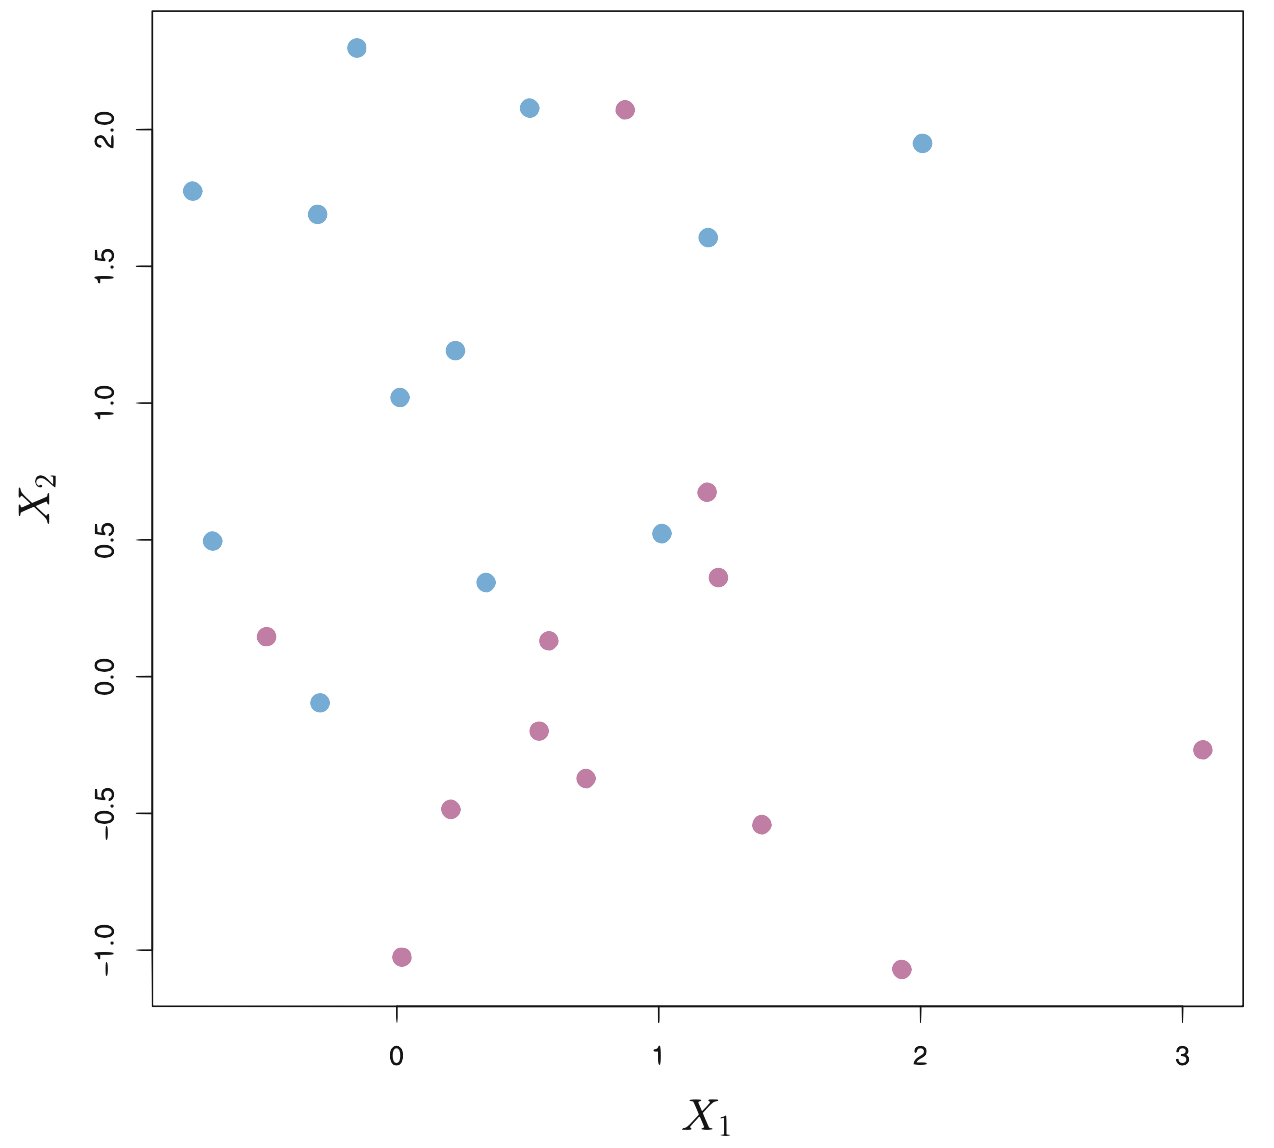
\includegraphics[width = .4\textwidth]{nonseperable.png}
	
	\vspace{-1em}
	\textbf{Data might not be linearly separable, in-which case the maximum margin classifier is not even defined.}
	\end{center}
	Less likely to be an issue when using a non-linear kernel. If $\bv{K}$ is full rank then perfect separation is always possible. And typically it is, e.g. for an RBF kernel or moderate degree polynomial kernel. 
\end{frame}


\begin{frame}
	\frametitle{hard-margin svm}
	\small
	While important in theory, hard-margin SVMs have a few critical issues in practice:
	\begin{center}
		\vspace{-1em}
		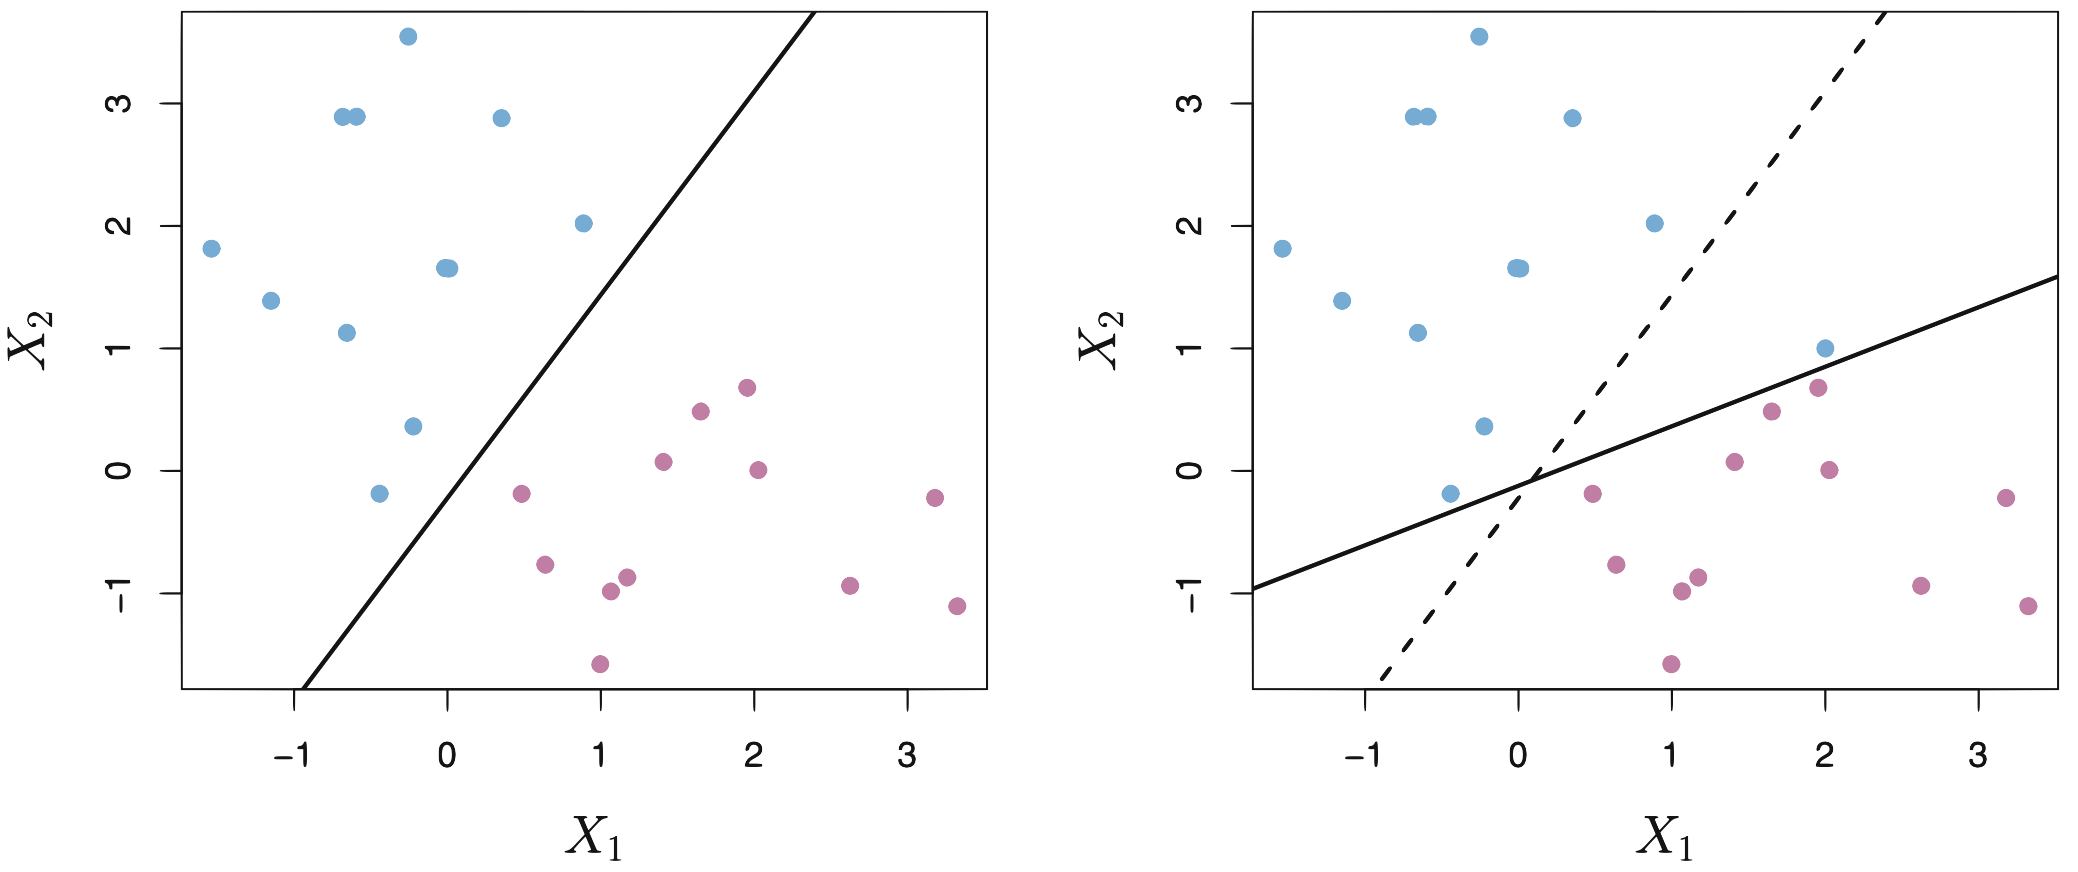
\includegraphics[width =\textwidth]{notrobust.png}
		
		\vspace{-.5em}
		\textbf{Hard-margin SVM classifiers are not robust.}
	\end{center}
\end{frame}

\begin{frame}
	\frametitle{soft-margin svm}
	\textbf{Solution}: Allow the classifier to make some mistakes! 
	
	\textbf{Hard margin objective:}
	\begin{align*}
	&\min_{\vec{\beta}} \|\vec{\beta}\|_2^2 & &\text{subject to}  & y_i\cdot\langle \vec{x}_i, \vec{\beta}\rangle &\geq 1 \text{ for all } i.
	\end{align*}
	
	\textbf{Soft margin objective:}
	\begin{align*}
	&\min_{\vec{\beta}} \|\vec{\beta}\|_2^2 \alert{+ C\sum_{i=1}^n\epsilon_i} & &\text{subject to}  & y_i\cdot\langle \vec{x}_i, \vec{\beta}\rangle &\geq 1 \alert{- \epsilon_i} \text{ for all } i.
	\end{align*}
	where $\epsilon_i \geq 0$ is a non-negative ``slack variable''. This is the magnitude of the ``error'' made on example $\vec{x}_i$. 
	
	$C \geq 0$ is a non-negative tuning parameter.
\end{frame}

\begin{frame}
	\frametitle{soft-margin svm}
	Example of a non-separable problem:
	\begin{center}
		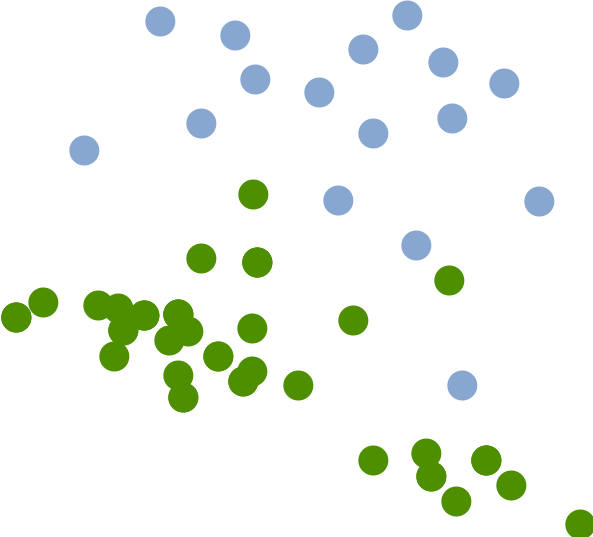
\includegraphics[width =.35\textwidth]{nonsep_example.png}
	\end{center}
\end{frame}

\begin{frame}
	\frametitle{soft-margin svm}
	\begin{center}
		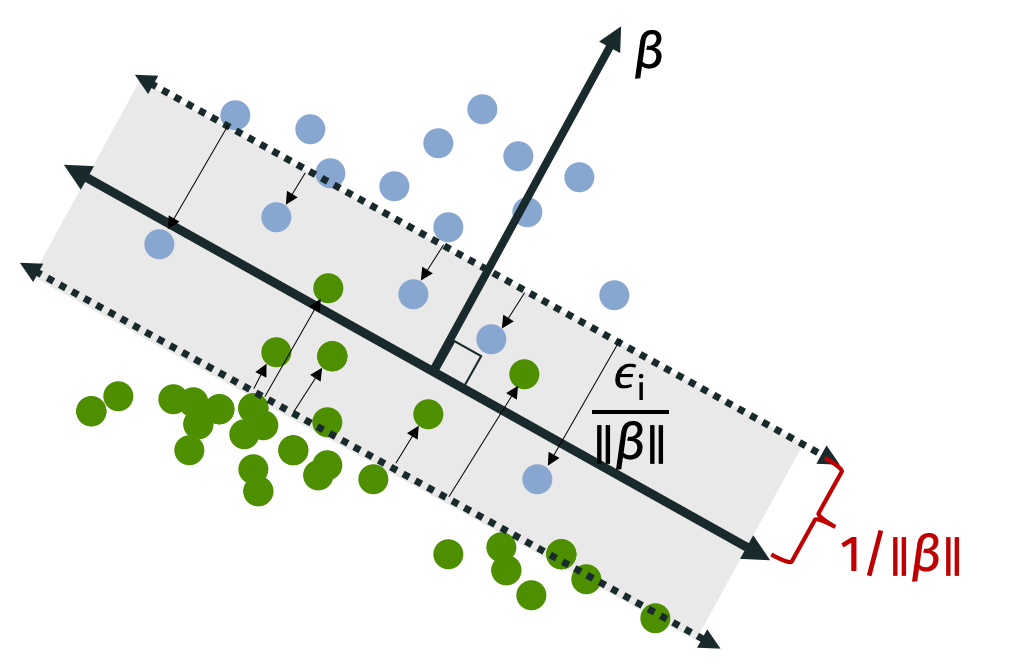
\includegraphics[width =.6\textwidth]{soft_margin.png}
	\end{center}
	\textbf{Soft margin objective:}
\begin{align*}
&\min_{\vec{\beta}} \|\vec{\beta}\|_2^2 + C\sum_{i=1}^n\epsilon_i & &\text{subject to}  & y_i\cdot\langle \vec{x}_i, \vec{\beta}\rangle &\geq 1 - \epsilon_i \text{ for all } i.
\end{align*}
\end{frame}

\begin{frame}
	\frametitle{soft-margin svm}
	\begin{center}
		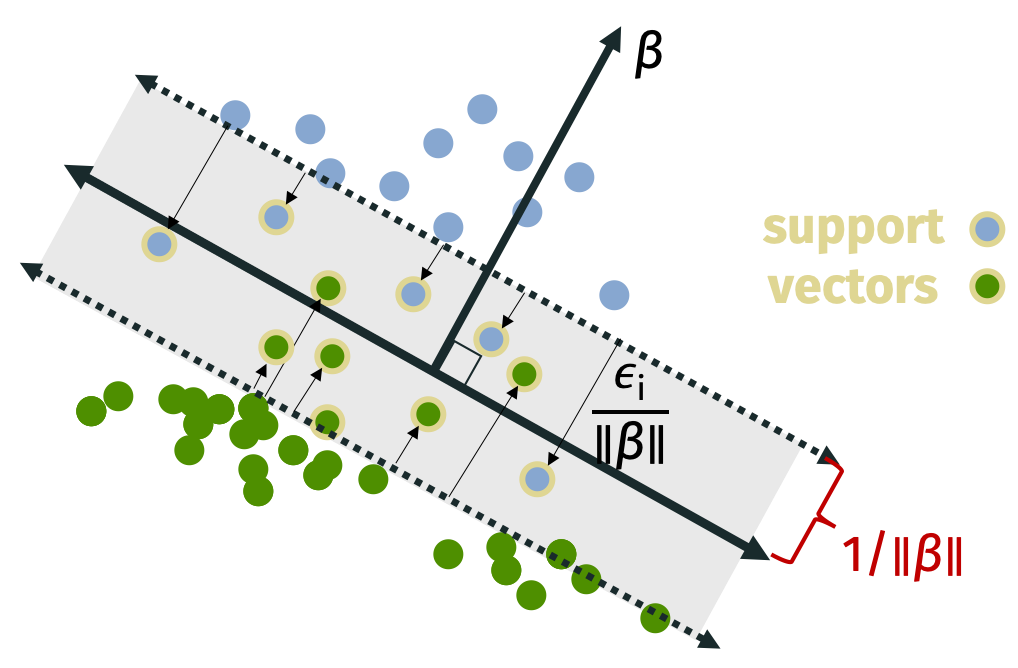
\includegraphics[width =.6\textwidth]{soft_support_vectors.png}
	\end{center}
	Any $\vec{x}_i$ with a non-zero $\epsilon_i$ is a \emph{support vector}. 
\end{frame}

\begin{frame}
	\frametitle{effect of c}
	\textbf{Soft margin objective:}
	\begin{align*}
	&\min_{\vec{\beta}} \|\vec{\beta}\|_2^2 + C\sum_{i=1}^n\epsilon_i.
	\end{align*}
	\begin{itemize}
		\item Large $C$ means penalties are punished more in objective $\Longrightarrow$ smaller margin, less support vectors.
		\item Small $C$ means penalties are punished less in objective $\Longrightarrow$ larger margin, more support vectors.
	\end{itemize}
When data is linearly separable, as $C\rightarrow \infty$ we will always get a separating hyperplane. A smaller value of $C$ might lead to a more robust solution. 
\end{frame}

\begin{frame}
	\frametitle{effect of c}
	\textbf{Example dataset:}
	\begin{center}
		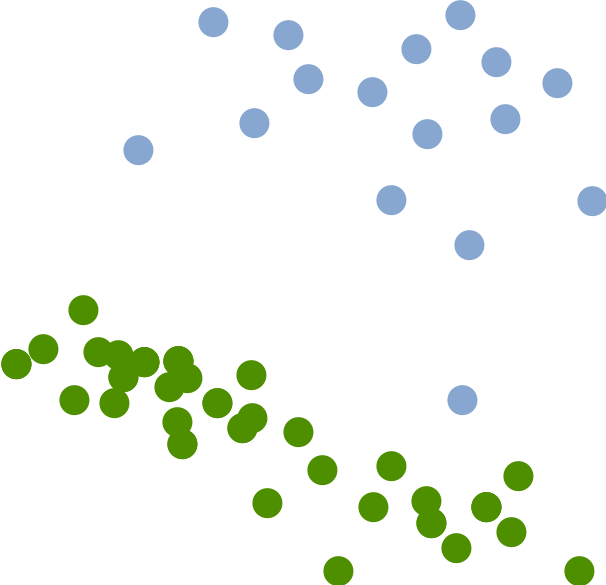
\includegraphics[width =.4\textwidth]{c_data.png}
	\end{center}
\end{frame}

\begin{frame}
	\frametitle{effect of c}
	\begin{center}
		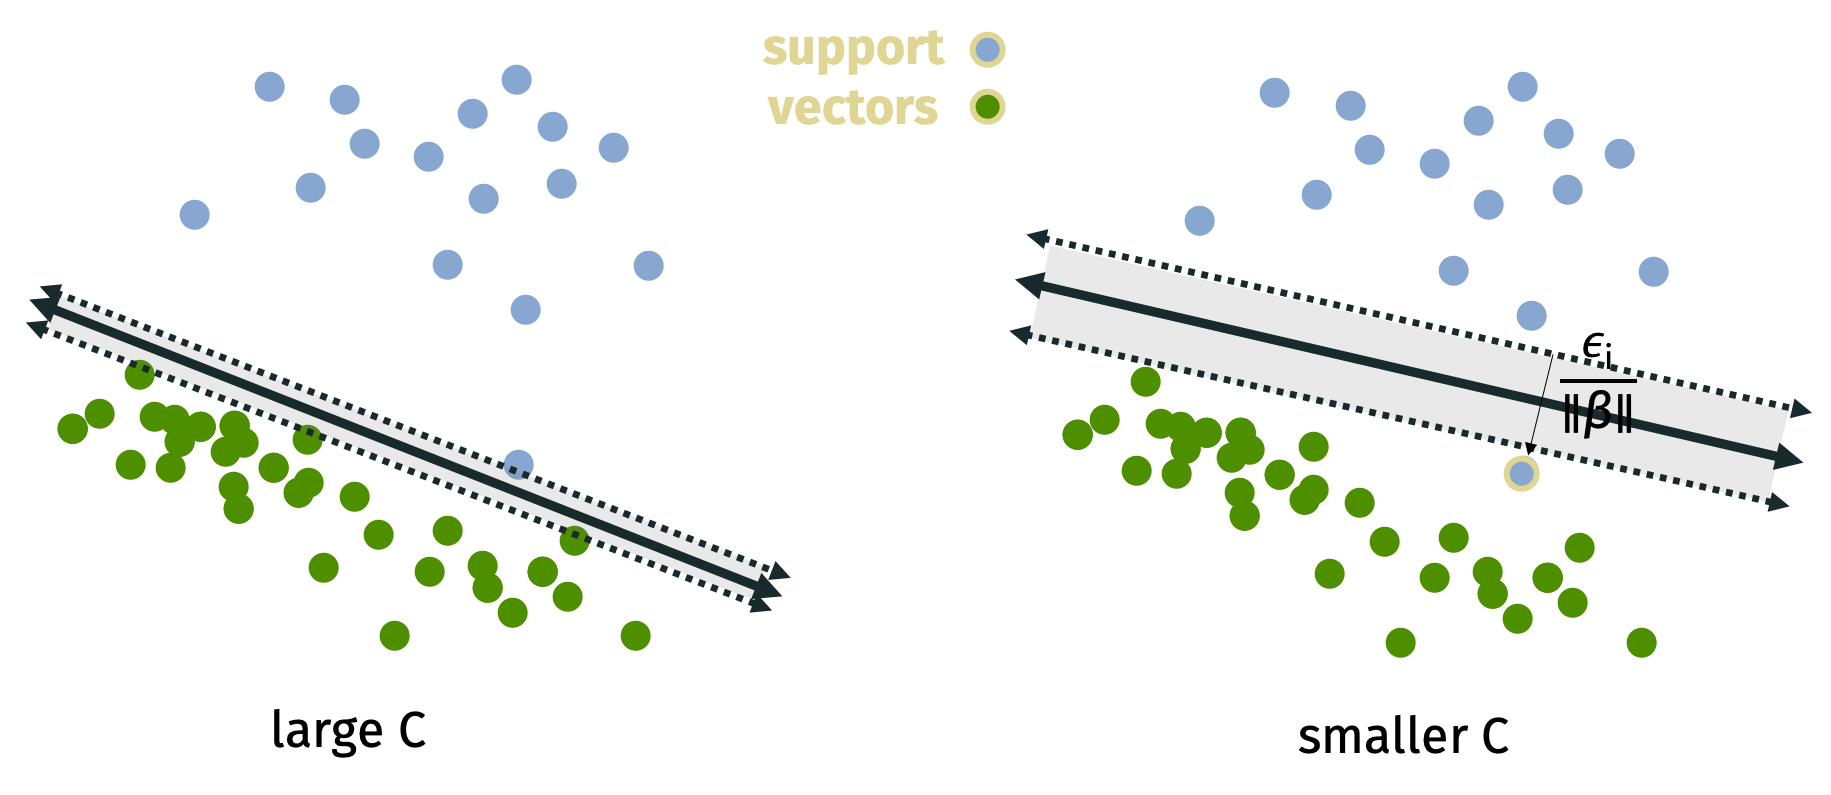
\includegraphics[width =.9\textwidth]{effect_c.png}
		
		The classifier on the right is intuitively more robust. So for this data, a smaller choice for $C$ might make sense. 
	\end{center}
\end{frame}

\begin{frame}
	\frametitle{dual formulation}
	\small
	\textbf{Reformulation of soft-margin objective:}
	\begin{align*}
	&\max_{\vec{\alpha}} \sum_{i=1}^n\alpha_i - \frac{1}{2}\sum_{i,j} y_iy_j\alpha_i\alpha_i \langle\vec{x}_i,\vec{x}_j\rangle - \frac{1}{2C}  \sum_{i=1}^n\alpha_i^2 \\
	&\text{subject to \,\,}  \alpha_i\geq 0, \,\,\,\sum_{i=1}^n\alpha_iy_i = 0.
	\end{align*}
	Obtained by taking the \emph{Lagrangian dual} of the objective. Beyond the scope of this class, but important for a few reasons:
	\begin{itemize}
		\item Objective only depends on inner products $\langle\vec{x}_i,\vec{x}_j\rangle$, which makes it clear how to combine the soft-margin SVM with a kernel. 
		\item Dual formulation can be solved faster in low-dimensions. 
		\item Possible to prove that $\alpha_i$ is only non-zero for the support vectors. When classifying a new data point, only need to compute inner products (or the non-linear kernel inner product) with this subset of training vectors. 
	\end{itemize}
\end{frame}


\begin{frame}
		\frametitle{comparison to logistic regression}
	\textbf{Some basic transformations of the soft-margin objective:}
	\begin{align*}
	&\min_{\vec{\beta}} \|\vec{\beta}\|_2^2 + C\sum_{i=1}^n\epsilon_i.
	\end{align*}
	\begin{align*}
		&\min_{\vec{\beta}} \|\vec{\beta}\|_2^2 + C\sum_{i=1}^n\max(0,1 -y_i\cdot\langle \vec{x}_i, \vec{\beta}\rangle).
	\end{align*}
	\begin{align*}
	&\min_{\vec{\beta}} \lambda\|\vec{\beta}\|_2^22 + \sum_{i=1}^n\max(0,1 -y_i\cdot\langle \vec{x}_i, \vec{\beta}\rangle).
	\end{align*}
	\begin{center}
		\alert{\textbf{These are all equivalent.}} $\lambda = 1/C$ is just another scaling parameter. 
	\end{center}
\end{frame}


\begin{frame}
	\frametitle{hinge loss}
	\textbf{Hinge-loss:} $\max(0,1-y_i\cdot\langle \vec{x}_i, \vec{\beta}\rangle)$. Recall that $y_i \in \{-1,1\}$. 
	\begin{center}
		\vspace{-1em}
		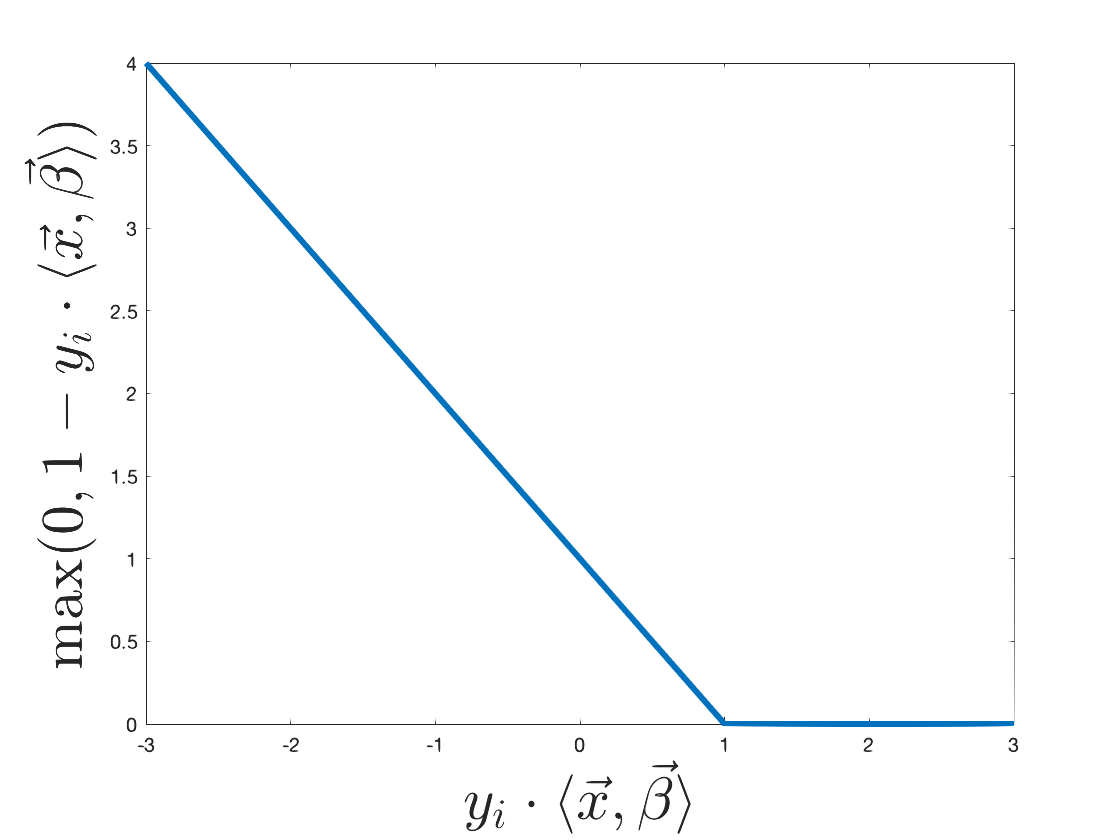
\includegraphics[width =.5\textwidth]{hinge.png}
	\end{center}
	\textbf{Soft-margin SVM:}
	\begin{align}
	\min_{\vec{\beta}} \left[\sum_{i=1}^n \max(0,1-y_i\cdot\langle \vec{x}_i, \vec{\beta}\rangle) + \lambda \|\vec{\beta}\|_2^2\right].
	\end{align}
\end{frame}

\begin{frame}
	\frametitle{comparison to logistic regression}
	Compare this to the logistic regression loss (slightly reformulated for $y_i\in \{-1,1\}$): 
	\begin{align*}
	\sum_{i=1}^n -\log(1 - \frac{1}{1-e^{y_i\cdot\langle \vec{x}_i, \vec{\beta}\rangle}}\rangle
	\end{align*}
	\begin{center}
		\vspace{-1em}
		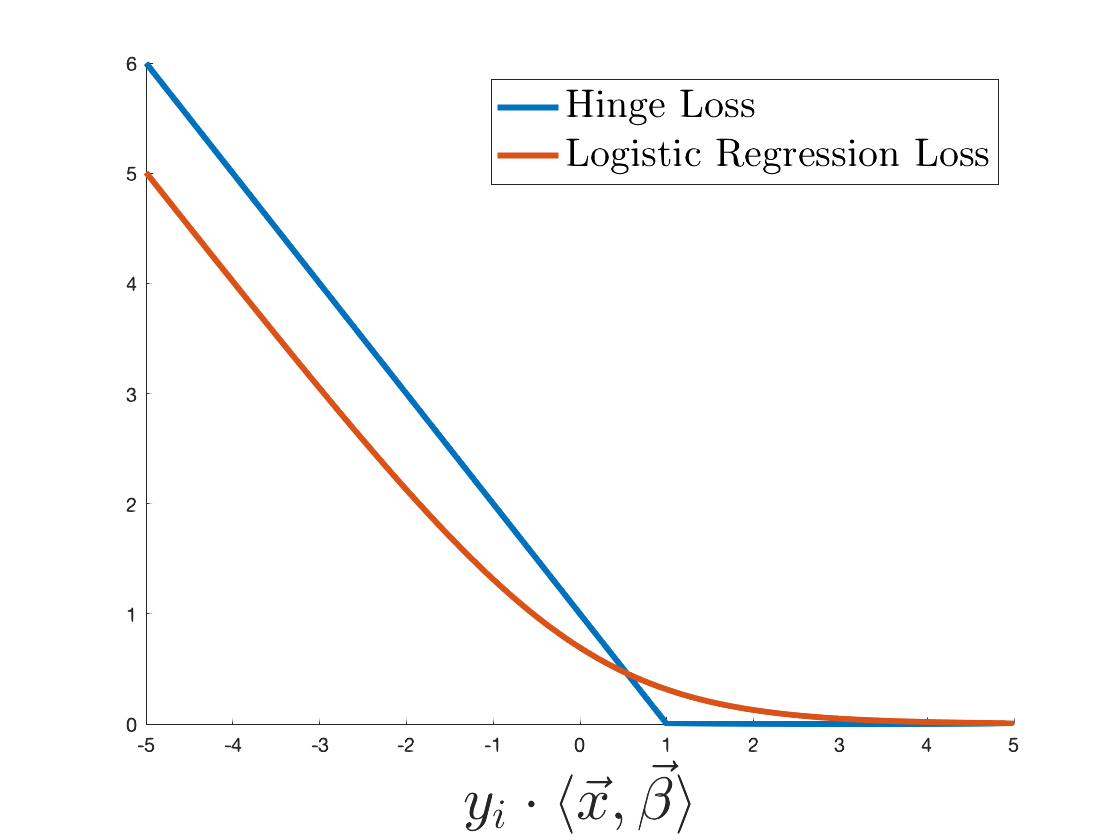
\includegraphics[width =.6\textwidth]{hinge_vs_log.png}
	\end{center}
\end{frame}

\begin{frame}
	\frametitle{comparison to logistic regression}
	So, in the end, the function minimized when finding $\vec{\beta}$ for the standard \textbf{soft-margin SVM} is \emph{very similar} to the objective function minimized when finding $\vec{\beta}$ using \textbf{logistic regression with $\ell_2$ regularization.} Sort of...
	\begin{center}
		\vspace{-1em}
		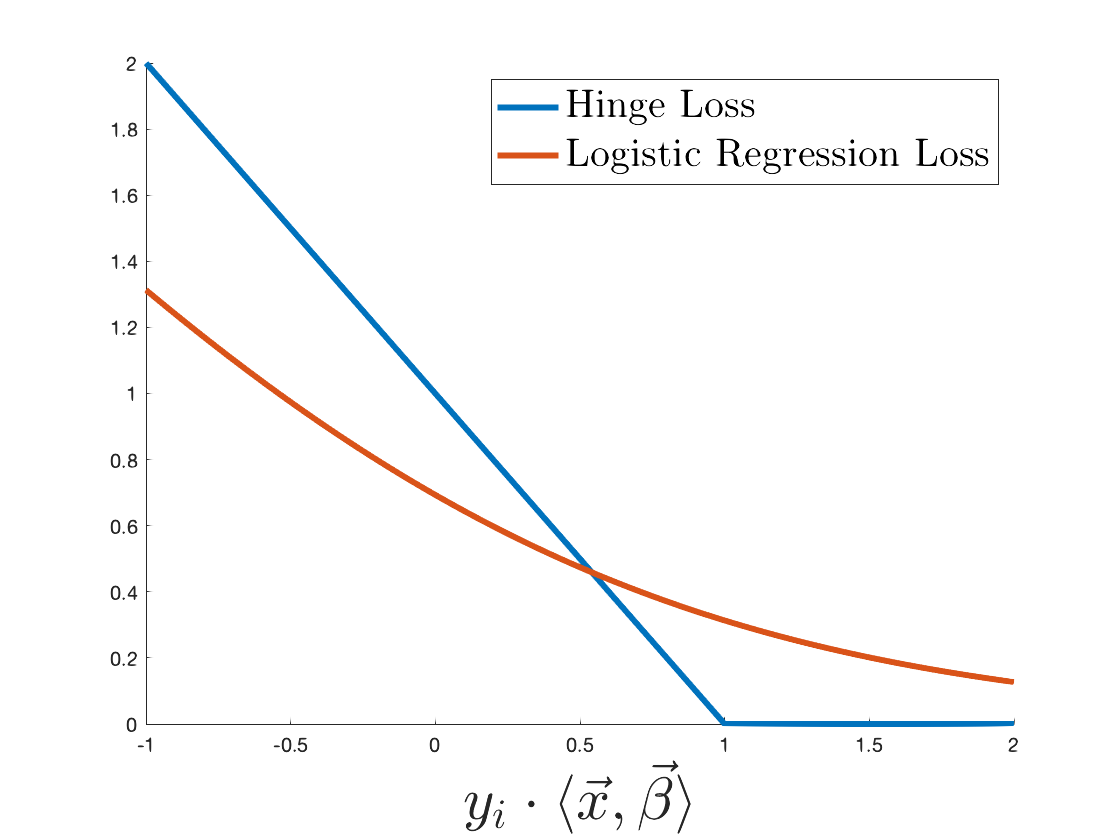
\includegraphics[width =.4\textwidth]{zoomed_in.png}
	\end{center}
	Both functions can be optimized using first-order methods like gradient descent. This is now a common choice for large problems.
\end{frame}

\begin{frame}
	\frametitle{comparison to logistic regression}
	The jury is still out on how different these methods are...
	\begin{center}
		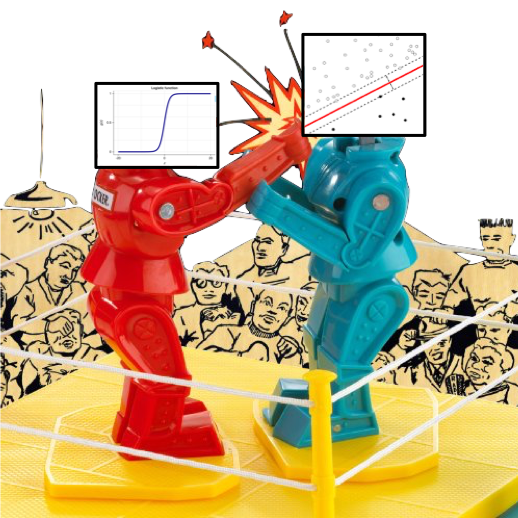
\includegraphics[width=.4\textwidth]{faceoff.png}
	\end{center}
	\begin{itemize}
		\item Work through \texttt{demo\_mnist\_svm.ipynb}. 
		\item Then complete lab \texttt{lab\_mnist\_partial.ipynb}.
	\end{itemize}
\end{frame}


\end{document} 






